\documentclass[a2paper, 12pt]{article}
\usepackage[font={huge, bf}]{caption}
\usepackage{fontspec}
\setmainfont{Arial}
\usepackage{subcaption}
\usepackage{graphicx}
\usepackage{tikz}
\usepackage{tikzsymbols}
\usetikzlibrary{calc,patterns,shapes.geometric}
\usepackage{float}
\usepackage{pdflscape}
\usepackage{geometry}
\geometry{landscape, margin=2cm}
\captionsetup[subfigure]{justification=justified,singlelinecheck=false}
\pagestyle{empty}

\def\centerarc[#1](#2)(#3:#4:#5){\draw[#1] ($(#2)+({#5*cos(#3)},{#5*sin(#3)})$) arc (#3:#4:#5);}

\begin{document}
	\vspace*{\fill}
	\begin{figure}[!htbp]
		\centering
		\begin{subfigure}[b]{0.48\textwidth}
			\caption{Figure 1}
			\centering
			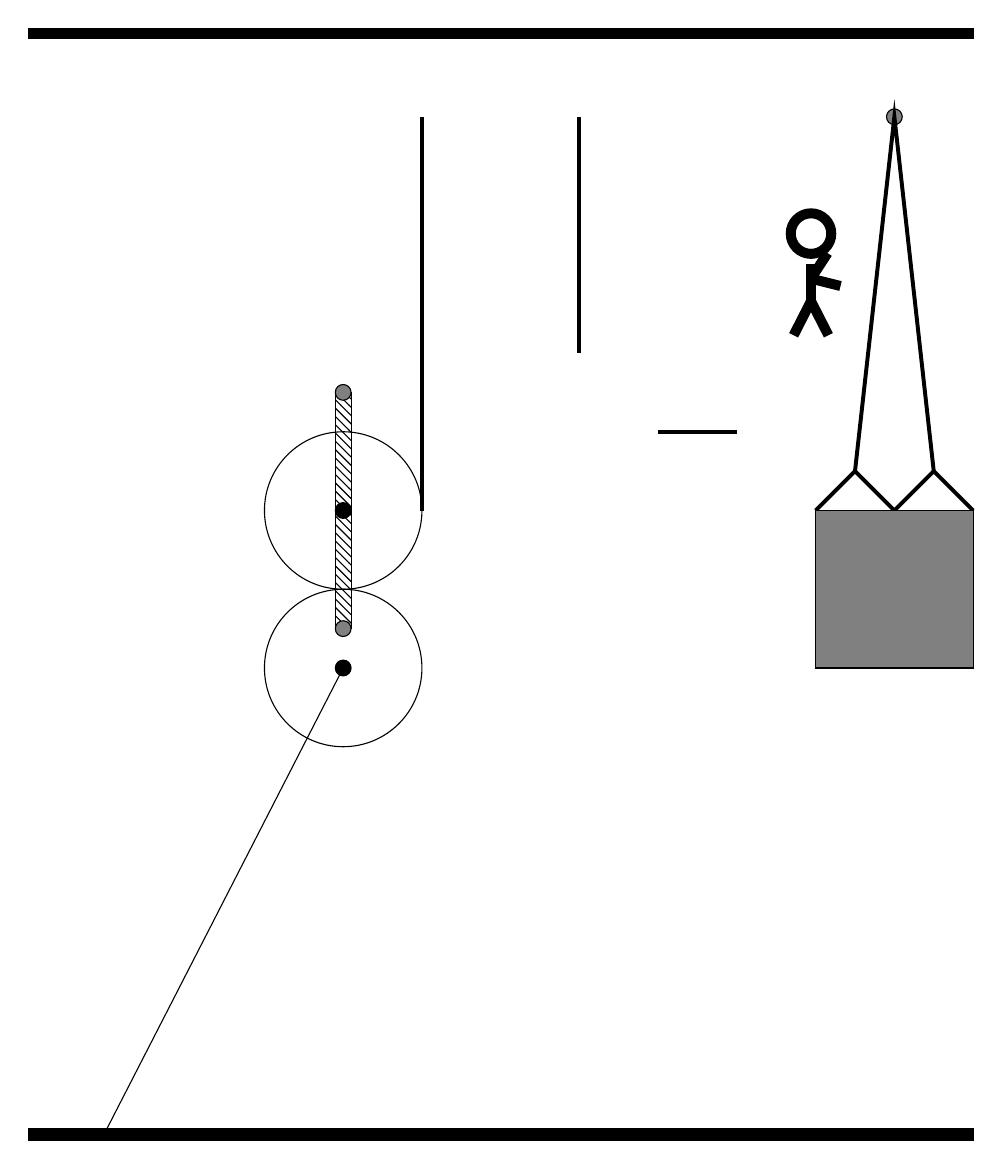
\begin{tikzpicture}
				\draw[fill=black] (-4, 14) rectangle (8, 14.125);
				
				\draw (0,6) circle (1);
				\draw[fill=black] (0,6) circle (0.1);
				\draw (-3,0.15) -- (0,6);
				
				\draw (0,8) circle (1);
				\draw[fill=black] (0,8) circle (0.1);
				\draw[pattern=north west lines, pattern color=black] (-0.1,9.5) rectangle (0.1,6.5);
				\draw[fill=black!50] (0,9.5) circle (0.1);
				\draw[fill=black!50] (0,6.5) circle (0.1);
				
				\draw[fill=black!50] (7,13) circle (0.1);
				\draw[line width=0.5mm](6.5,8.5) -- (7,13) --  (7.5,8.5);
				\draw[line width=0.5mm](6,8) --  (6.5,8.5) -- (7,8) -- (7.5,8.5) -- (8,8);
				\draw[fill=black!50] (6, 8) rectangle (8, 6);
				
				\draw[line width = 0.5mm] (1,8) -- (1,13);
				\centerarc[line width = 0.5mm](2,13)(0:180:1);
				\draw[line width = 0.5mm] (3,13) -- (3,10);
				\centerarc[line width = 0.5mm](4,10)(270:180:1);
				\draw[line width = 0.5mm] (4,9) -- (5,9);
				
				\node at (6, 11) {\scriptsize \Strichmaxerl[10][166][57]};
				
				\draw[fill=black] (-4, 0) rectangle (8, 0.15);
			\end{tikzpicture}
		\end{subfigure}
		\hfill
		\begin{subfigure}[b]{0.48\textwidth}
			\caption{Figure 2}
			\centering
			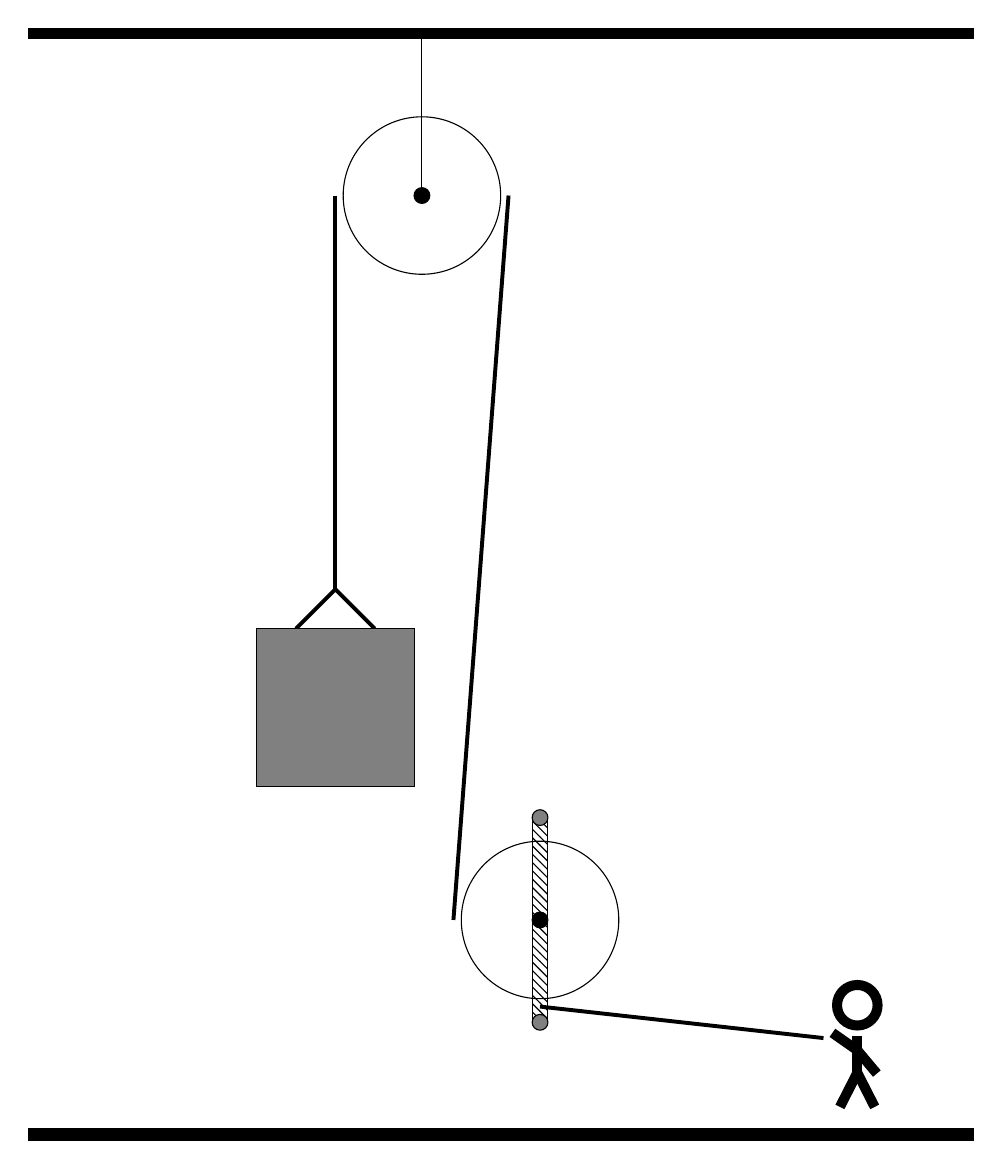
\begin{tikzpicture}
				\draw[fill=black] (-4, 14) rectangle (8, 14.125);
				
				\draw (1, 12) circle (1);
				\draw[fill=black] (1, 12) circle (0.1);
				\draw (1, 14) -- (1, 12);
				
				\draw[fill=white](2.5, 2.8) circle (1);
				\draw[fill=black] (2.5, 2.8) circle (0.1);
				\draw[pattern=north west lines, pattern color=black] (2.4, 4.1) rectangle (2.6, 1.5);
				\draw[fill=black!50] (2.5, 4.1) circle (0.1);
				\draw[fill=black!50] (2.5, 1.5) circle (0.1);
				
				\draw[line width=0.5mm] (-0.6, 6.5) -- (-0.1, 7.0) -- (0.4, 6.5);
				\draw[fill=black!50] (-1.1, 6.5) rectangle (0.9, 4.5);
				
				\draw[line width=0.5mm] (-0.1, 12) -- (-0.1, 7.0);
				\centerarc[line width=0.5mm](1, 12)(0:180:1.1);
				\draw[line width=0.5mm](2.1, 12) -- (1.4, 2.8);
				\centerarc[line width=0.5mm](2.5, 2.8)(180:270:1.1);
				\draw[line width=0.5mm](2.5, 1.7) -- (6.1, 1.3);
				
				\node at (6.5, 1.2) {\scriptsize \Strichmaxerl[10][-35][-50]};
				
				\draw[fill=black] (-4, 0) rectangle (8, 0.15);
			\end{tikzpicture}
		\end{subfigure}
	\end{figure}
		\vspace*{\fill}
\end{document}